\chapter{Requisiti Funzionali}
\label{ch:requisitiFunzionali}

Di seguito vengono riportati i requisiti funzionali (\texttt{RF}) del programma ``SatisTrento'' tramite \textit{Use Case Diagram} (\texttt{UCD}) progettati usando il linguaggio \texttt{UML}.

\section{\underline{Utente non loggato}}
    Di seguito i requisiti associati all'Utente non loggato:
    \begin{itemize}
        \item \textbf{RF1}: Visualizzazione città
        \item \textbf{RF2}: Interazione con la mappa
        \item \textbf{RF3}: Visualizzazione zona
        \item \textbf{RF4}: Elenco strutture
        \item \textbf{RF5}: Multi lingua
        \item \textbf{RF6}: Login
    \end{itemize}
    \begin{figure}[H]
        \centering
        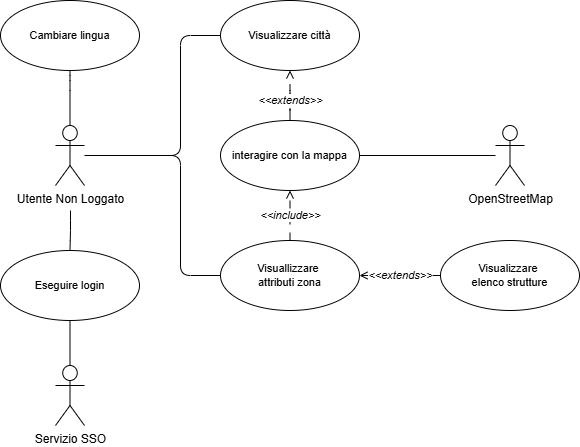
\includegraphics[width=0.8\textwidth]{UseCase_diagrams/NonLoggato.drawio.png}
        \caption{\textit{Use Case Diagram} dell'Utente non loggato}
    \end{figure}

    \subsection{\textit{Use Case} RF1: Visualizzare città}
        \subsubsection{Riassunto}
            Questo \textit{Use Case} descrive come l'utente può visualizzare gli attributi e la mappa della città
        \subsubsection{Descrizione}
            \begin{itemize}
                \item Il sistema mostra nella parte sinistra dello schermo gli attributi demografici e riguardanti la soddisfazione della città
                \item Il sistema mostra nella parte destra dello schermo la mappa della città suddivisa nella zona selezionata (Estensione 1)
            \end{itemize}
        \subsubsection{Estensioni}
            \begin{itemize}
                \item La tipologia di zona selezionata di default è quella dei quartieri
            \end{itemize}
    
    \subsection{\textit{Use Case} RF2: Interagire con la mappa}
        \subsubsection{Riassunto}
            Questo \textit{Use Case} descrive come l'utente può interagire con la mappa
        \subsubsection{Descrizione}
            \begin{itemize}
                \item L'utente non loggato posiziona il cursore all'interno dello spazio dedicato alla mappa
                \item Se l'utente utilizza la rotella del mouse oppure uno dei pulsanti presenti in uno degli angoli della mappa
                \item Attraverso le funzionalità fornite da \texttt{OpenStreetMap}\footnote{
                    \label{note:osm}
                    $ \text{\texttt{OpenStreetMap}}^{\text{\textregistered}} $ è basato su \textit{dati aperti}, rilasciato con licenza \href{https://opendatacommons.org/licenses/odbl/}{\textit{Open Data Commons Open Database License} (\texttt{ODbL})} da \href{https://osmfoundation.org/}{\textit{\texttt{OpenStreetMap} Foundation} (\texttt{OSMF})}. Per ulteriori informazioni si rimanda al sito ufficiale: \url{https://www.openstreetmap.org/}
                } la mappa ingrandisce o diminuisce la dimensione dello zoom (Eccezione 1)
                \item Se l'utente preme e trascina il cursore
                \item Attraverso le funzionalità fornite da \texttt{OpenStreetMap}\footref{note:osm} la mappa sposta il focus centrale in funzione del cursore (Eccezione 2)
                \item Se l'utente non loggato seleziona una delle zone all'interno della visuale della mappa (Estensione 1)
                \item Il sistema posiziona il focus centrale della mappa al centro della zona selezionata e ne modifica successivamente lo zoom, il colore e lo spessore dei bordi
                \item Il sistema passa successivamente allo \textit{Use Case} ``Visualizzare zona'' della sezione scelta(Eccezione 3)
            \end{itemize}
        \subsubsection{Eccezioni}
            \begin{enumerate}
                \item Nel caso in cui l'utente non loggato cercasse di aumentare o diminuire lo zoom oltre ai limiti imposti, il sistema deve bloccare la nuova modifica allo zoom
                \item Nel caso in cui l'utente non loggato cercasse di spostare il focus centrale oltre ai limiti della città, il sistema deve bloccare la nuova modifica allo spostamento del focus centrale
                \item Nel caso in cui l'utente avesse i permessi necessari, il sistema passerà allo \textit{Use Case} ``Accesso completo agli attributi'' della sezione scelta invece che allo allo \textit{Use Case} ``Visualizzare zona'' della sezione scelta
            \end{enumerate}
        \subsubsection{Estensioni}
            \begin{enumerate}
                \item Nel caso in cui l'utente cliccasse su di una zona già selezionata questa riporterebbe allo \textit{Use Case} ``Visualizzare città''
                \item L'utente, selezionando il pulsante presente nell'angolo della mappa, potrà visualizzare un menù pop-up e successivamente modificare la tipologia di zona visualizzabile all'interno della mappa.
                Nel caso in cui l'utente avesse i permessi necessari, sarà inoltre possibile cambiare la tipologia di visualizzazione da mappa a tabella.
            \end{enumerate}
    
    \subsection{\textit{Use Case} RF3: Visualizzare zona}
        \subsubsection{Riassunto}
            Questo \textit{Use Case} descrive come l'utente può visualizzare la zona selezionata della città
        \subsubsection{Descrizione}
            \begin{enumerate}
                \item L'utente seleziona una zona geografica per la quale ricevere maggiori informazioni
                \item Il sistema mostra nella parte sinistra dello schermo la mappa centrata sul centro della zona selezionata
                \item Il sistema mostra nella parte destra dello schermo gli attributi demografici e riguardanti la soddisfazione della zona della città selezionata
            \end{enumerate}

    \subsection{\textit{Use Case} RF4: Visualizzare elenco strutture}
        \subsubsection{Riassunto}
            Questo \textit{Use Case} descrive come l'utente può accedere e visualizzare l'elenco delle strutture che forniscono un servizio al cittadino
        \subsubsection{Descrizione}
            \begin{enumerate}
                \item Se l'utente seleziona uno degli attributi presenti a schermo (Eccezione 1)
                \item Il sistema presenta a schermo, ove prima erano presenti gli attributi riguardanti la zona selezionata, una tabella contenente una lista numerata di strutture che offrono il servizio selezionato in precedenza
                \item Il sistema deve successivamente segnalare sulla mappa la posizione delle varie strutture, attraverso un segnalino contenente il numero identificativo presente in tabella della struttura
            \end{enumerate}
        \subsubsection{Eccezioni}
            \begin{enumerate}
                \item Nel caso in cui per una tipologia di dato non fossero presenti strutture il sistema non deve fare nulla
            \end{enumerate}
        \subsubsection{Estensioni}
            \begin{enumerate}
                \item Nel caso in cui l'utente cliccasse il pulsante per chiudere la tabella il sistema tornerà alla visualizzazione della zona selezionata in precedenza
            \end{enumerate}

    \subsection{\textit{Use Case} RF5: Cambiare lingua}
        \subsubsection{Riassunto}
            Questo \textit{Use Case} descrive come l'utente può cambiare la lingua dei vari testi presenti nel programma
        \subsubsection{Descrizione}
            \begin{enumerate}
                \item L'utente preme sul menù a tendina presente nella header e seleziona la sezione riguardante la modifica della lingua
                \item Il sistema presenterà a schermo un menù pop-up contenente la lista di lingue per le quali è disponibile la traduzione
                \item Se l'utente seleziona la lingua e clicca il pulsante di conferma (Eccezione 1 e 2)
                \item Il sistema ricarica la pagina selezionata con i testi nella lingua selezionata
            \end{enumerate}
        \subsubsection{Eccezioni}
            \begin{enumerate}
                \item Nel caso in cui l'utente non loggato selezionasse e confermasse la lingua già selezionata, il sistema deve chiudere il pop-up senza apportare alcuna modifica
            \end{enumerate}

    \subsection{\textit{Use Case} RF6: Eseguire login}
        \subsubsection{Riassunto}
            Questo \textit{Use Case} descrive come l'utente non loggato può eseguire il login
        \subsubsection{Descrizione}
            \begin{enumerate}
                \item L'utente preme sul menù a tendina presente all'interno della header e seleziona la sezione riguardante il login
                \item Il sistema reindirizza l'utente alla pagina del service provider della provincia di Trento dal quale potrà accedere al login tramite sistema \texttt{SSO}
                \item Il sistema \texttt{SSO} verifica l'identità dell'utente in questione e la ritorna al sistema (Eccezione 1)
                \item Il sistema controlla che per l'identità certificata dal sistema \texttt{SSO} esista un'account collegato (Eccezione 1)
                \item Il sistema assegna dunque un'identità all'utente assegnandogli il ruolo di proprietà
                \item Il sistema successivamente al login sostituisce l'icona del login con l'immagine profilo dell'account al quale si ha fatto l'accesso e reindirizza l'utente allo \textit{Use Case} ``visualizzare città''
            \end{enumerate}
        \subsubsection{Eccezioni}
            \begin{enumerate}
                \item Nel caso in cui l'autenticazione fallisse o non vi fossero account collegati il sistema ritorna alla pagina dalla quale si ha provato a fare il login
            \end{enumerate}


\section{\underline{Utente sondaggista}}
    Di seguito i requisiti associati all'Utente sondaggista:
    \begin{itemize}
        \item \textbf{RF7}: Logout
        \item \textbf{RF8}: Visualizzazione sondaggi
        \item \textbf{RF9}: Gestione sondaggi
        \item \textbf{RF10}: Visualizzazione voti
        \item \textbf{RF11}: Gestione voti
    \end{itemize}
    \begin{figure}[H]
        \centering
        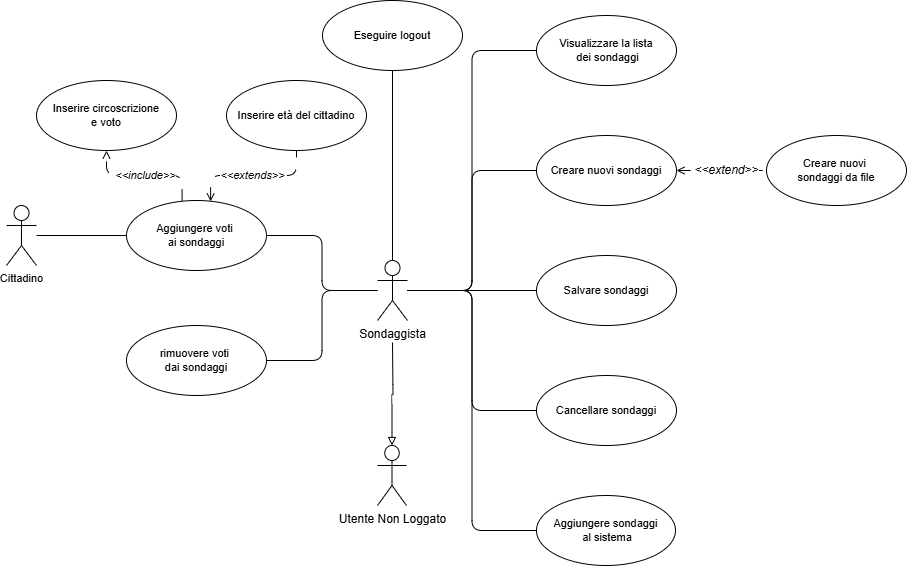
\includegraphics[width=0.8\textwidth]{UseCase_diagrams/Sondaggista.drawio.png}
        \caption{\textit{Use Case Diagram} dell'Utente sondaggista}
    \end{figure}

    \subsection{\textit{Use Case} RF7: Logout}
        \subsubsection{Riassunto}
            Questo \textit{Use Case} descrive come l'utente può fare logout
        \subsubsection{Descrizione}
            \begin{enumerate}
                \item L'utente sondaggista preme sul menù a tendina presente all'interno della header e seleziona la sezione riguardante il logout
                \item Il sistema scollega lo user dall'account al quale era collegato riportandolo allo stato di utente non loggato, infine 
                ricarica la pagina riportando l'utente alla 'visualizzazione città'
            \end{enumerate}

    \subsection{\textit{Use Case} RF8: Visualizzare i sondaggisti}
        \subsubsection{Titolo}
            Questo \textit{Use Case} descrive come l'utente sondaggista può visualizzare i sondaggi e le interfacce per gestirli
        \subsubsection{Descrizione}
            \begin{enumerate}
                \item Il sistema mostra nel riquadro in alto a sinistra dello schermo l'interfaccia per la creazione di nuovi sondaggi con relative caselle di testo e pulsante per la creazione
                \item Il sistema mostra nel riquadro in basso a sinistra dello schermo l'interfaccia per il caricamento dei sondaggi attraverso pulsante o ``\textit{drag and drop}''
                \item Il sistema mostra nel riquadro in alto a destra dello schermo l'elenco dei sondaggi non ancora caricati, o in fase di caricamento, a sistema con relativo stato della sessione (Eccezione 1)
                \item Il sistema mostra nel riquadro in basso a destra dello schermo l'elenco dei sondaggi già caricati a sistema con relativo stato di caricamento e stato di verifica dei dati inseriti (Eccezione 1)
            \end{enumerate}
        \subsubsection{Eccezioni}
            \begin{enumerate}
                \item Nel caso in cui non fossero presenti sondaggi all'interno di uno degli elenchi il sistema mostrerà a schermo un messaggio per avvisare che tale sezione risulta vuota
            \end{enumerate}

    \subsection{\textit{Use Case} RF9: Gestione sondaggi}
%        \begin{figure}[H]
%            \includegraphics[width=0.8\textwidth]{% Bisogna inserire il path della foto del boss}
%        \end{figure}

    \subsection{\textit{Use Case} RF10: Visualizzare i voti}
        \subsubsection{Titolo}
            Questo \textit{Use Case} descrive come l'utente sondaggista può visualizzare i voti e le interfacce per gestirli
        \subsubsection{Descrizione}
            \begin{enumerate}
                \item Il sistema mostra nella parte sinistra dello schermo un riassunto del numero di voti presenti all'interno del sondaggio e in basso una tabella riassuntiva riguardante il numero di voti ricevuti per quartiere
                \item Il sistema mostra nel riquadro in alto a destra dello schermo l'interfaccia per il caricamento dei voti con le corrispettive caselle di testo
                \item Il sistema mostra nel riquadro in basso a destra dello schermo l'interfaccia per la gestione dei sondaggi
                \item Il sistema mostra nel riquadro in basso al centro dello schermo l'elenco dei voti caricati in precedenza, su ogni voto è inoltre presente l'id, l'ora al quale è stato caricato il voto e infine il pulsante per eliminarlo (Eccezione 1)
            \end{enumerate}
        \subsubsection{Eccezioni}
            \begin{enumerate}
                \item Nel caso in cui non fossero presenti voti all'interno della lista il sistema mostrerà a schermo un messaggio per avvisare che tale sezione risulta vuota
            \end{enumerate}

    \subsection{\textit{Use Case} RF11: Gestione voti}
%        \begin{figure}[H]
%            \includegraphics[width=0.8\textwidth]{% Bisogna inserire il path della foto del boss}
%        \end{figure}


\section{\underline{Utente analista}}
    Di seguito i requisiti associati all'Utente analista:
    \begin{itemize}
        \item \textbf{RF7}: Logout
        \item \textbf{RF12}: Interazione con la tabella
        \item \textbf{RF13}: Accesso completo agli attributi
        \item \textbf{RF14}: Analisi attraverso storici
    \end{itemize}
    \begin{figure}[H]
        \centering
        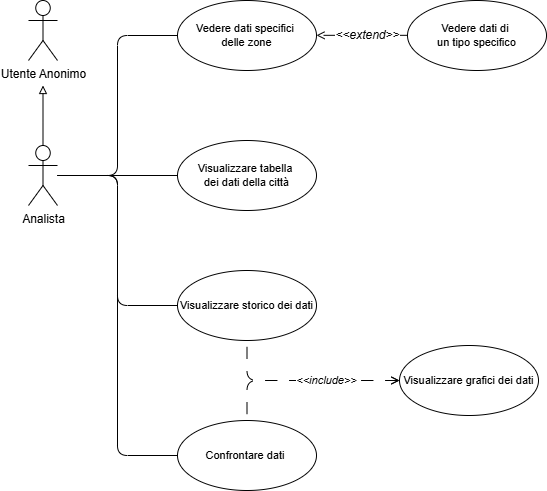
\includegraphics[width=0.8\textwidth]{UseCase_diagrams/Analista.drawio.png}
        \caption{\textit{Use Case} Diagram dell'Utente analista}
    \end{figure}

    \subsection{\textit{Use Case} RF7: Logout}
        \subsubsection{Riassunto}
            Questo \textit{Use Case} descrive come l'utente può fare logout
        \subsubsection{Descrizione}
            \begin{enumerate}
                \item L'utente analista preme sul menù a tendina presente all'interno della header e seleziona la sezione riguardante il logout
                \item Il sistema scollega lo user dall'account al quale era collegato riportandolo allo stato di utente non loggato, infine 
                ricarica la pagina riportando l'utente alla 'visualizzazione città'
            \end{enumerate}

    \subsection{\textit{Use Case} RF12: Interazione con la tabella}
        \subsubsection{Titolo}
            Questo \textit{Use Case} descrive come l'utente analista visualizzerà e potrà interagire con la tabella
        \subsubsection{Descrizione}
            \begin{enumerate}
                \item L'utente analista posiziona il cursore all'interno dello spazio dedicato alla tabella
                \item Se l'utente utilizza la rotella del mouse
                \item La tabella scorre gli elementi presenti all'interno della tabella (Eccezione 1)
                \item Se l'utente seleziona uno degli attibuti all'interno della riga di intestazione della tabella
                \item Il sistema ordina le tuple presenti all'interno della tabella in base al dominio dell'attributo
                \item Se l'utente seleziona l'attributo contenente il nome di una delle zone presenti all'interno del comune
                \item Il sistema passa dalla visualizzazione tramite tabella a quella tramite mappa
                \item il sistema sposta il focus centrale della mappa al centro della zona selezionata e ne modifica successivamente lo zoom, il colore e lo spessore dei bordi
                \item Il sistema passa successivamente allo \textit{Use Case} ``Accesso completo agli attributi'' della sezione scelta
            \end{enumerate}
        \subsubsection{Eccezioni}
            \begin{enumerate}
                \item Nel caso in cui l'utente analista cercasse di scorrere gli elementi della lista oltre ai limiti imposti, il sistema deve bloccare il nuovo tentativo di scorrimento
            \end{enumerate}
        \subsubsection{Estensioni}
            \begin{enumerate}
                \item L'utente, selezionando il pulsante presente nell'angolo della tabella, potrà visualizzare un menù pop-up.Successivamente potrà modificare la tipologia di zona presente all'interno della tabella oppure cambiare la tipologia di visualizzazione da tabella a mappa
            \end{enumerate}

    \subsection{\textit{Use Case} RF13: Accesso completo agli attributi}
        \subsubsection{Titolo}
            Questo \textit{Use Case} descrive come l'utente analista può visualizzare, accedere e navigare agli attributi completi riguardanti ogni zona
        \subsubsection{Descrizione}
            \begin{enumerate}
                \item L'utente seleziona una zona geografica per la quale ricevere maggiori informazioni
                \item Il sistema mostra nella parte sinistra dello schermo la mappa centrata sul centro della zona selezionata
                \item Il sistema mostra nella parte destra dello schermo la categoria di attributi riguardanti la zona selezionata con al di sopra le icone ed il titolo delle varie categorie di attributi selezionabili (Estensione 2)
                \item L'utente seleziona la categoria di attributi che vuole visualizzare (Eccezione 1)
                \item Il sistema mostra, ove prima erano presenti gli attributi della precedente categoria, gli attributi appartenenti alla nuova categoria selezionata
            \end{enumerate}
        \subsubsection{Eccezioni}
            \begin{enumerate}
                \item Se si seleziona la categoria di attributi già selezionata il sistema non deve fare nulla
            \end{enumerate}
        \subsubsection{Estensioni}
            \begin{enumerate}
                \item Questo \textit{Use Case} estende lo \textit{Use Case} ``Visualizzazione Zona'' dell'utente non loggato
                \item La categoria di attributi selezionata di default è quella degli attributi generali
            \end{enumerate}

    \subsection{\textit{Use Case} RF14: Analisi attraverso storici}
        \subsubsection{Titolo}
            Questo \textit{Use Case} descrive come l'utente analista può visualizzare e interagire con gli storici
        \subsubsection{Descrizione}
            \begin{enumerate}
                \item Il sistema mostra a fianco degli attributi presenti all'interno dello \textit{Use Case} ``Accesso completo agli attributi'' il grafico rappresentante l'andamento nel tempo di tale attributo
                \item L'utente seleziona il grafico
                \item Il sistema sposta l'attributo selezionato e successivamente posiziona al centro il grafico modificandone le dimensioni (Eccezione 1)
                \item Se l'utente posiziona il cursore all'interno del grafico
                \item Il sistema mostrerà tramite messaggio a comparsa lo stato dell'attributo nell'istante di tempo selezionato
            \end{enumerate}
        \subsubsection{Eccezioni}
            \begin{enumerate}
                \item Nel caso in cui per un'attributo non fossero reperibili sufficienti dati non sarà presente la propria rappresentazione tramite grafico
            \end{enumerate}


\section{\underline{Utente circoscrizione}}
    Di seguito i requisiti associati all'Utente circoscrizione:
    \begin{itemize}
        \item \textbf{RF7}: Logout
        \item \textbf{RF15}: Visualizzazione richieste
        \item \textbf{RF16}: Gestione richieste
        \item \textbf{RF17}: Gestione ruoli Circoscrizione
        \item \textbf{RF18}: Modifica informazioni servizi Circoscrizione
    \end{itemize}
    \begin{figure}[H]
        \centering
        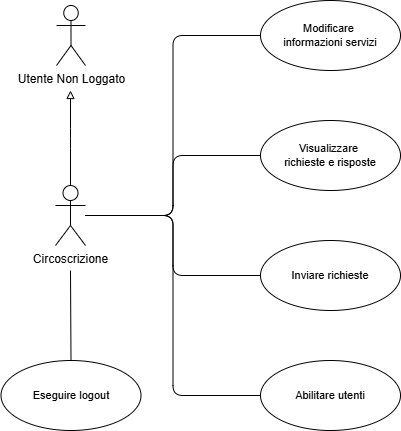
\includegraphics[width=0.8\textwidth]{UseCase_diagrams/Circoscrizione.drawio.png}
        \caption{\textit{Use Case} Diagram dell'Utente circoscrizione}
    \end{figure}

    \subsection{\textit{Use Case} RF7: Logout}
        \subsubsection{Riassunto}
            Questo \textit{Use Case} descrive come l'utente può fare logout
        \subsubsection{Descrizione}
            \begin{enumerate}
                \item L'utente circoscrizione preme sul menù a tendina presente all'interno della header e seleziona la sezione riguardante il logout
                \item Il sistema scollega lo user dall'account al quale era collegato riportandolo allo stato di utente non loggato, infine 
                ricarica la pagina riportando l'utente alla 'visualizzazione città'
            \end{enumerate}

    \subsection{\textit{Use Case} RF15: Visualizzazione richieste}
        \subsubsection{Titolo}

        \subsubsection{Descrizione}
            \begin{enumerate}
                \item
            \end{enumerate}
        \subsubsection{Eccezioni}
            \begin{enumerate}
                \item
            \end{enumerate}
        \subsubsection{Estensioni}
            \begin{enumerate}
                \item
            \end{enumerate}

    \subsection{\textit{Use Case} RF16: Gestione richieste}
        \subsubsection{Titolo}
            
        \subsubsection{Descrizione}
            \begin{enumerate}
                \item 
            \end{enumerate}
        \subsubsection{Eccezioni}
            \begin{enumerate}
                \item
            \end{enumerate}
        \subsubsection{Estensioni}
            \begin{enumerate}
                \item
            \end{enumerate}

    \subsection{\textit{Use Case} RF17: Gestione ruoli Circoscrizione}
        \subsubsection{Titolo}
            
        \subsubsection{Descrizione}
            \begin{enumerate}
                \item 
            \end{enumerate}
        \subsubsection{Eccezioni}
            \begin{enumerate}
                \item 
            \end{enumerate}

    \subsection{\textit{Use Case} RF18: Modifica informazioni servizi Circoscrizione}
        \subsubsection{Titolo}
            
        \subsubsection{Descrizione}
            \begin{enumerate}
                \item 
            \end{enumerate}
        \subsubsection{Eccezioni}
            \begin{enumerate}
                \item 
            \end{enumerate}